\subsection{Results}

The percentage of Triangle Inequality failures was investigated for matrix pairs, $A, B \in M_n$ with varying entry types and dimension. For real ($M_n(\mathbb R)$) or integer ($M_n(\mathbb Z)$) type entries, the values range from $(-k, k)$, $k\in \mathbb Z$. For Gaussian integer ($M_n(\mathbb Z[i])$) or complex ($M_n(\mathbb C)$) type entries, the values are of the form $a+bi$, where $a,b$ range from $(-k, k)$, $k\in \mathbb Z$. Sample failure percentages for each entry types were calculated from 100,000 randomly chosen pairs within a fixed entry range $(-k, k)$. True failure percentages were also calculated for pairs $A, B \in M_2(\mathbb Z)$ by exhaustively determining all possible pairs (with replacement) with entry ranges $(-k, k)$, $k \geq 7 \in \mathbb Z$. (\autoref{fig:sample_true_fail_rates_n2_varied_types_ranges})
\begin{figure}[H]
    \centering
    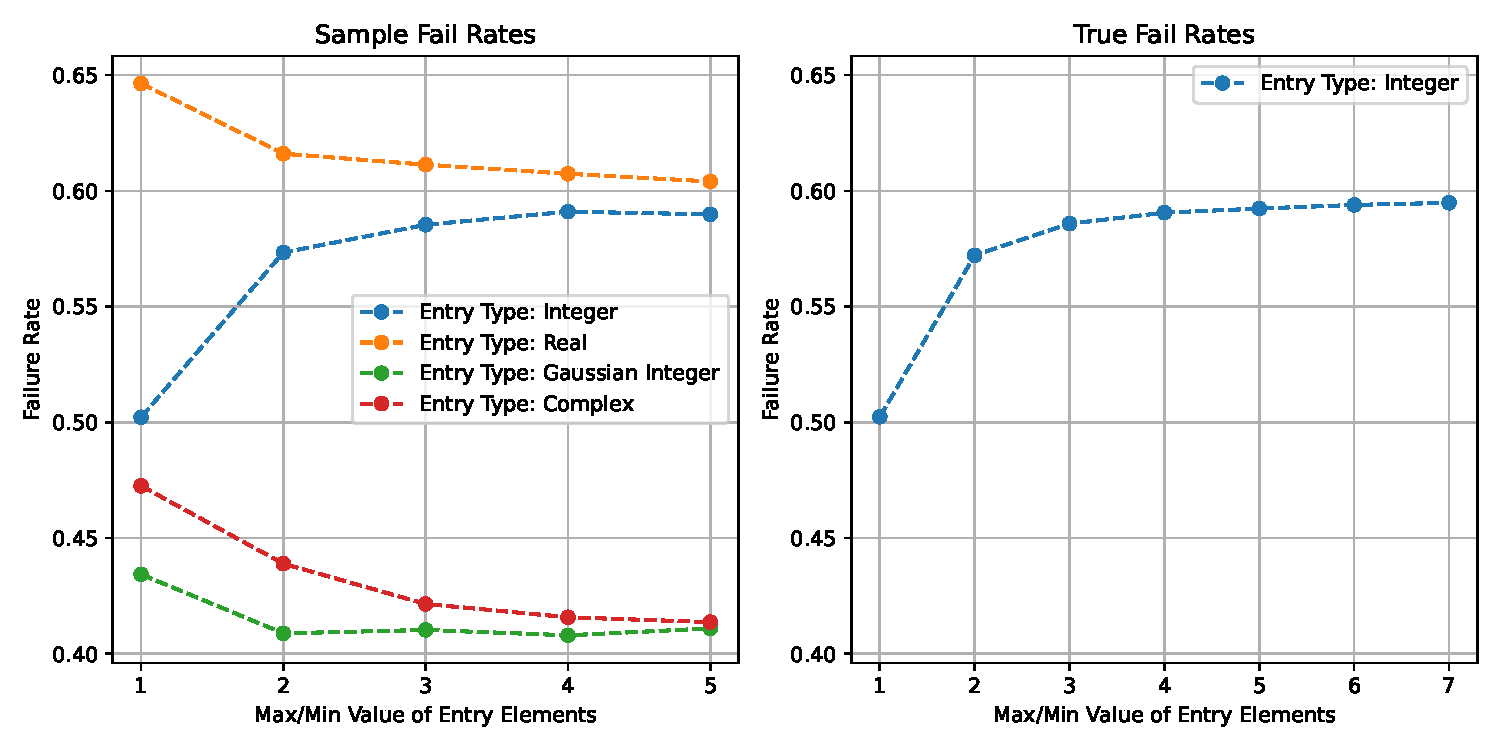
\includegraphics[width=\textwidth]{assets/sample_true_fail_rates_n2_varied_types_ranges.pdf}
    \caption{Comparison of sample and true triangle inequality failure rates of $M_2$. Each sample point contains 100,000 randomly chosen matrix pairs, with standard tolerance}\label{fig:sample_true_fail_rates_n2_varied_types_ranges}
\end{figure}

The effect of increasing the dimensions of the matrix pairs were also investigated. Sample Failure Rates for all entry types at a standard tolerance of $10^{-7}$ were produced for $2\leq n\leq 5$. (\autoref{fig:sample_fail_rate_varied_n_type_range})

\begin{figure}[H]
    \centering
    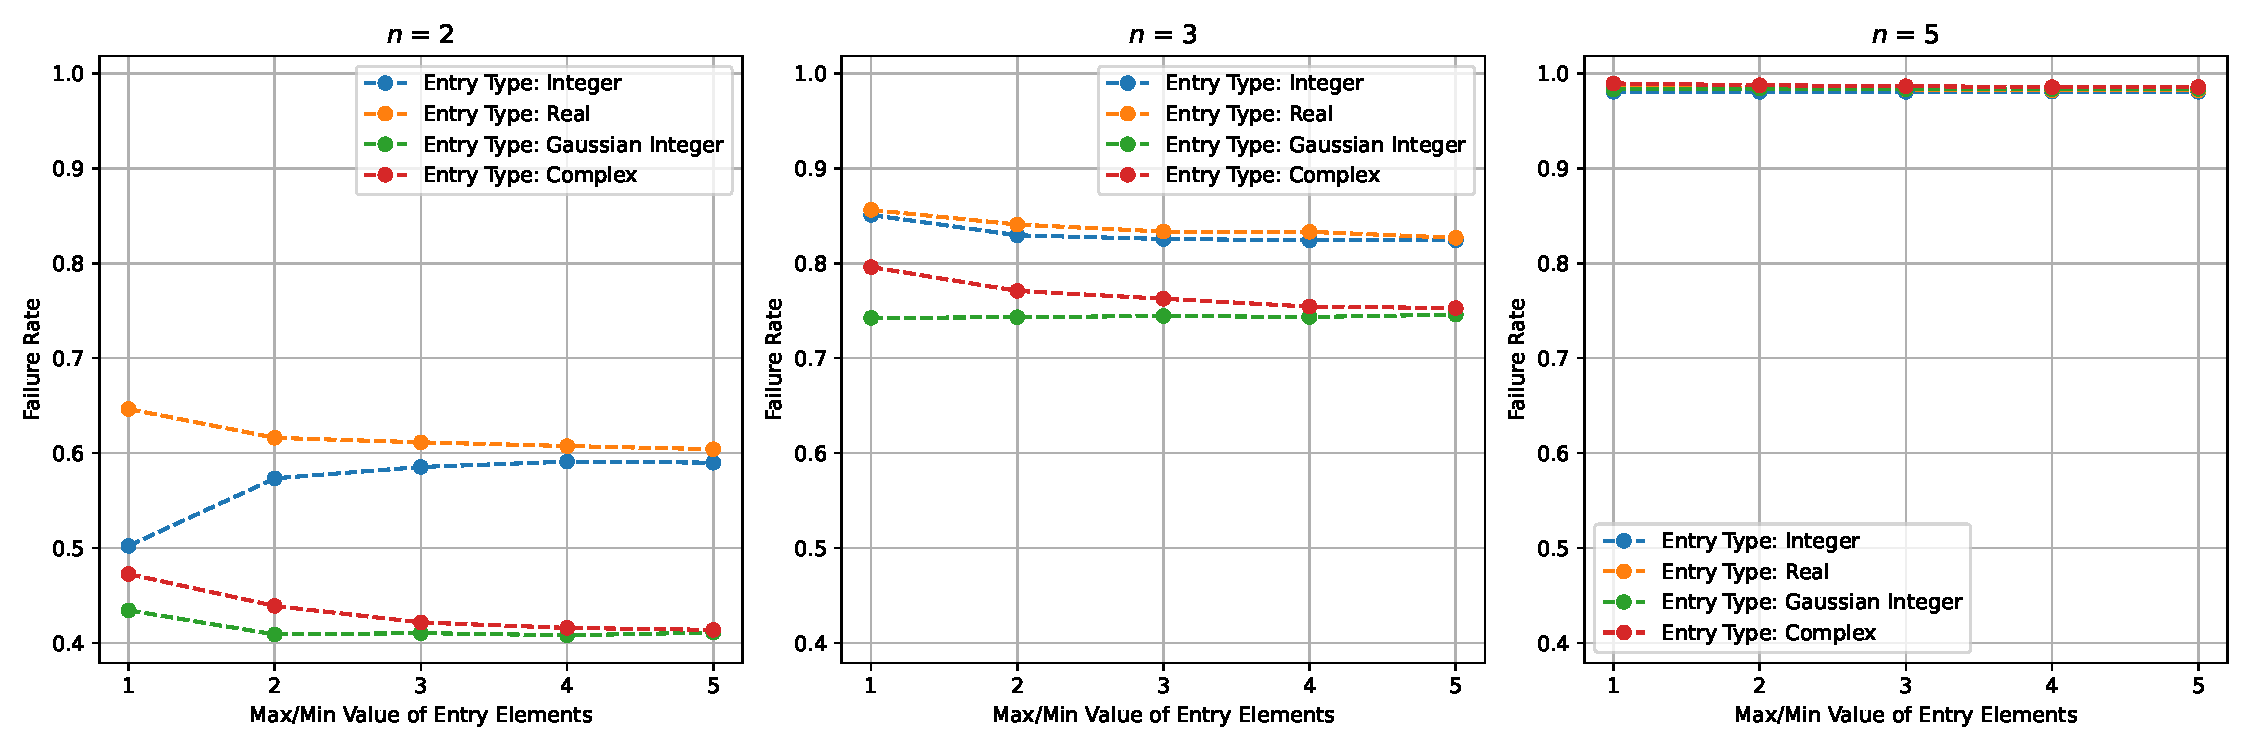
\includegraphics[width=\textwidth]{./assets/sample_fail_rate_varied_n_type_range.pdf}
    \caption{Changes in fail rate as $n$ increases. Each sample point contains 100,000 randomly chosen matrix pairs, with standard tolerance}\label{fig:sample_fail_rate_varied_n_type_range}
\end{figure}